\documentclass{article}

% Language setting
% Replace `english' with e.g. `spanish' to change the document language
\usepackage[spanish]{babel}

% Set page size and margins
% Replace `letterpaper' with `a4paper' for UK/EU standard size
\usepackage[letterpaper,top=2cm,bottom=2cm,left=3cm,right=3cm,marginparwidth=1.75cm]{geometry}

% Useful packages
\usepackage{amsmath}
\usepackage{graphicx}
\usepackage[colorlinks=true, allcolors=blue]{hyperref}
\usepackage[settings]{markdown}

\title{Trabajo Final Calculo}
\author{Leider Santiago Cortes, Juan Felipe Monsalve Vargas}
\date{Diciembre 5, 2022}

\begin{document}
\maketitle
%\begin{abstract}
%Your abstract.
%\end{abstract}

\section{Introducción}
Documento correspondiente con el Trabajo Final, nota del último corte de la materia Calculo II, en el cual debemos dar explicación y aplicar ejemplos a los siguientes temas.
\begin{itemize}
  \item Coordenadas cilíndricas.
  \item Coordenadas esféricas.
  \item Teorema de Stokes.
  \item Operador laplaciano.
\end{itemize}

Todo esto tiene como objetivo que usando cambio de coordenadas y la regla de la cadena en varias variables hallar la forma del operador laplaciano en coordenadas cilíndricas o esféricas.


\section{Coordenadas Cilíndricas}
Es un sistema de coordenadas, usado en aquellos casos donde los problemas tienen simetría tipo cilindro, ya que por ejemplo al hacer integrales se puede simplificar mucho el problema con la conversión de coordenadas cartesianas a coordenadas polares. El sistema de coordenadas cilíndricas es la versión en 3D de las coordenadas polares \ref{fig:polares_graf}


\begin{figure}[htp]
    \centering
    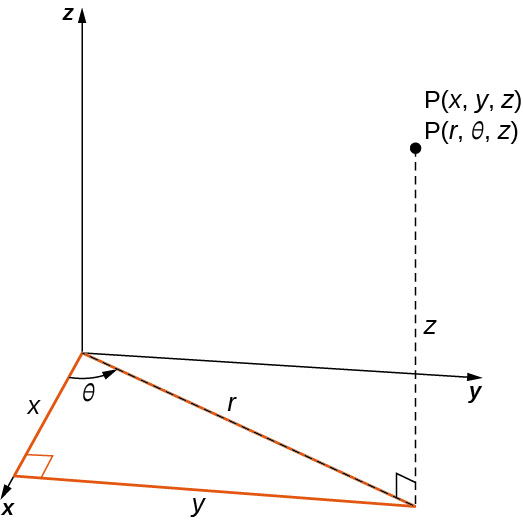
\includegraphics[width=0.5\textwidth]{polares_graf.jpg}
    \caption{El gráfico muestra la manera de graficar coordenadas cilíndricas.}
    \label{fig:polares_graf}
\end{figure}

Un punto $ P $ cualquiera en coordenadas cilíndricas se representar por $ (\rho ,\varphi ,z) $ (Mirar la imagen {fig:polares_graf}):

\begin{itemize}
  \item \textbf{\textit{$ \rho $ radio}}: definido como la distancia del punto $ P $ al eje $ $, también conocida como la proyección del radiovector con el plano $XY$. Varía entre $ 0\leq \rho <\infty  $
  \item \textbf{\textit{$ \varphi $ Coordenada azimutal}}: definida como el ángulo que forma con el eje $ X $ la proyección del radiovector sobre el plano $ XY $. Varía entre: $ \qquad 0\leq \varphi <2\pi $
  \item \textbf{\textit{$ z $ Coordenada vertical}}: Punto en el eje $z$. Varía entre: $  \qquad -\infty <z<\infty $
\end{itemize}


\subsection{Conversión entre coordenadas cartesianas y cilíndricas}
Para convertir entre coordenadas polares y cartesianas debemos aplicar las siguientes ecuaciones:
 $$ x=\rho \cos \varphi ,\qquad y=\rho \sin \varphi ,\qquad z=z $$


\section{Coordenadas esféricas}
that are natural for describing positions on a sphere or spheroid. Define theta to be the azimuthal angle in the xy-plane from the x-axis with 0<=theta<2pi (denoted lambda when referred to as the longitude), phi to be the polar angle (also known as the zenith angle and colatitude, with phi=90 degrees-delta where delta is the latitude) from the positive z-axis with 0<=phi<=pi, and r to be distance (radius) from a point to the origin. This is the convention commonly used in mathematics.

\begin{figure}[htp]
    \centering
    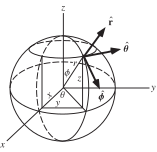
\includegraphics[width=0.5\textwidth]{spheric coord.svg}
    \caption{El gráfico muestra la manera de graficar coordenadas esferícas.}
    \label{fig:spheric_coord}
\end{figure}

\subsection{How to add Citations and a References List}

You can simply upload a \verb|.bib| file containing your BibTeX entries, created with a tool such as JabRef. You can then cite entries from it, like this: \cite{greenwade93}. Just remember to specify a bibliography style, as well as the filename of the \verb|.bib|. You can find a \href{https://www.overleaf.com/help/97-how-to-include-a-bibliography-using-bibtex}{video tutorial here} to learn more about BibTeX.


\bibliographystyle{alpha}
\bibliography{sample}

\end{document}